\documentclass[a4paper,10pt]{scrartcl}
\usepackage[top=2.5cm, bottom=2cm, left=2.5cm, right=2.5cm]{geometry}

% UTF-8 support
\usepackage[utf8]{inputenc}

% german and english language support
\usepackage[english,ngerman]{babel}

% more math symbols
\usepackage{amsmath}

% advanced tables
\usepackage{tabularx}

% hide the hyperlinks
\usepackage[hidelinks]{hyperref}

% no newpage after include
\usepackage{newclude}

% fancy graphics
\usepackage{graphicx}

% more customizable captions
\usepackage{caption}

% nice font
\usepackage{lmodern}

% ???
\usepackage{textcomp}
% \usepackage[onehalfspacing]{setspace}
% \linespread{0.95}

% Tikz for designing graphics
\usepackage{tikz}
\usetikzlibrary{positioning}

% code
\usepackage{listings}
\lstset{ %
  frame=single,	                   % adds a frame around the code
  language=Python,                 % the language of the code
  numbers=left,                    % where to put the line-numbers; possible values are (none, left, right)
  stepnumber=1,                    % the step between two line-numbers. If it's 1, each line will be numbered
}

% hyperref / hyperlink settings
\usepackage{hyperref}
\hypersetup{
colorlinks,
citecolor=black,
filecolor=black,
linkcolor=black,
urlcolor=black
}

% renew some commands
\newcommand{\bold}{\textbf}
\renewcommand{\arraystretch}{1.5}
\newcommand{ \rarrow }{\( \rightarrow \)}

% redefine some parameters
\setlength\parindent{0pt}
\setlength\parskip{10pt}
\setlength{\footskip}{30pt}
\setcounter{tocdepth}{3}

%%% MAIN DOCUMENT BEGINS HERE %%%

\begin{document}

% titlepage settings
\title{Galaxy Generation}
\subtitle{Jugend Forscht \the\year}
\author{ Emile Hansmaennel \texttt{ emile.hansmaennel@gmail.com }}
\date{\today}

% generate the title using the informations given above
\maketitle

% include a nice image
\begin{figure}[h]
  \centering
  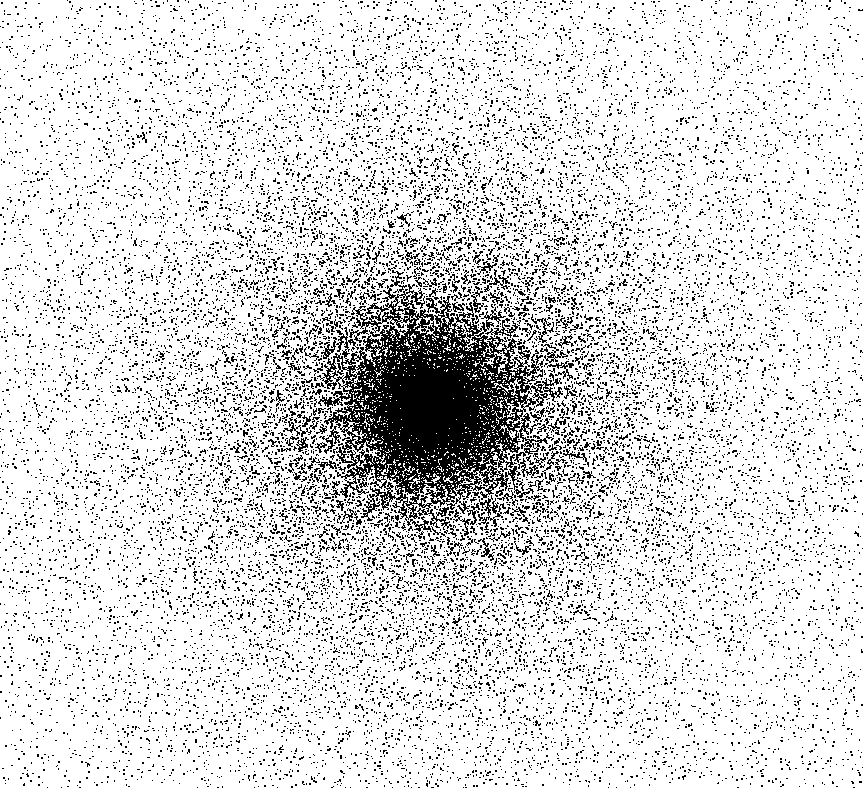
\includegraphics[width=120mm, trim={0 8.5cm 0 8.5cm}, clip]{figs/galaxy}
  \captionsetup{labelformat=empty}
  \caption{}
 \end{figure}

% include the abstract
\begin{abstract}
\include*{docs/1_kurzfassung}
\end{abstract}

% don't insert a page number on the first page
\thispagestyle{empty}
\clearpage
\newpage
\setcounter{page}{1}

% generate a table of contents
\tableofcontents
\newpage

\section{Einleitung} \label{Einleitung}
% Nach meinem letzten Jugend-Forscht Projekt ergab sich die Möglichkeit ein
Praktikum im Zentrum für Astronomie in Heidelberg zu absolvieren. Über die
social-media Platform Reddit stellte ich den kontakt mit Tim Tugendkat her
der zurzeit seinen PhD. in Physik an der Universität in Heidelberg macht.
Dieser ermöglichte es mir, die Physikalische Fakultät an einer Uni mal genauer
zu sehen und das täglich leben eines Physikers mitzuerleben.
\par
Während des Praktikums stellte ich fest das ich die im letzten Jahr erlerne Fähigkeit mit
Python\footnote{Programmiersprache} zu Programmieren und mit
Blender\footnote{3D Software Suite} umzugehen nutzen konnte um Galaxien
darzustellen.
Dies war insgesamt unglaublich Interessant und zeigte mir zum wiederholten mal:
Projekte sind sehr dazu geeignet um sich in neues einzuarbeiten oder neues
zu lernen und bieten einem ein Ziel welches man erreichen möchte was einem
immer genügend motivation bietet weiterzumachen.
\par
Eine frage die ich mir öfters gestellt habe war warum man eigentlich Galaxien
simuliert? Wäre es nicht einfacher einfach in den Himmel zu gucken und
die bereits bestehenden Galaxien zu beobachten?
Nach kurzer recherche lag die Antwort auf der Hand: Galaxien brauchen mehrere
Millionen Jahre um sich zu entwickeln, also kann man ihre Entwicklung als
normaler Mensch nicht in dem Umfang beobachten, um dann daraus schlüsse zu
ziehen. Daher simuliert man die Galaxien und kann dann somit vorhersagen oder
herrausfinden wie die Galaxien entstanden sind bzw. was mit ihnen passieren
wird.

\subsection{Themen}

\begin{itemize}
  \item Generierung von Elliptischen Galaxien
  \item Generierung von einem Dark-Matter Halo um die Elliptische Galaxie
  \item Stauchung und Streckung des Dark-Matter mit beinflussung der eigentlichen Galaxie
  \item Beschleunigung des generierungsprozesses mithilfe einer sogennanten ''lookup-table``
  \item Aufbau eines neuronalen Netzes für die unbeaufsichtigte Generation von Galaxien
  \item Generation von Spiralgalaxien
\end{itemize}

\subsection{Motivation}

Ich habs einfach mal getan...

\include*{docs/2_einleitung}
\newpage

\section{Hauptteil} \label{Hauptteil}
% 
% \paragraph{ \( \Phi \) }
%
% \begin{equation}
%   \Phi(r) = - \frac{4\pi G \rho_0 R_s^3}{r} \ln ( 1+ \frac{r}{R_s} )
% \end{equation}
%
% with the limits
%
% \begin{equation}
%   \lim_{r\to \infty} \Phi=0
% \end{equation}
%
% and
%


\subsection{Generierung der Elliptischen Galaxien}
\subsubsection{Das Navarro-Frenk-White Profil}

Das Navarro-Frenk-White profil (NFW-profil) ist im grunde genommen eine Funktion
die einem die Warscheinlichkeit das ein Stern an einer bestimmten position ist
liefert.
Die Funktion ist im allgemeinen wie folgt aufgebaut:

\begin{equation} \label{eq:NFW_profile}
  \rho_{NFW}(r) = \frac{ 1 }{ \sqrt{ 2 \pi } \cdot \sigma } \cdot
  \exp \left( \frac{ -\phi(r) }{ \sigma^{ 2 } } \right)
\end{equation}

\begin{equation*}
  \phi(r) = \frac{ 4\pi \cdot G \cdot f_{0} \cdot R_{s}^3 }{ r } \cdot
  ln{ \left( 1 + \frac{ r }{ R_{s} } \right) }
\end{equation*}

Um die Formel (\ref{eq:NFW_profile}) einfach zu beschreiben kann man sie sich
wie folgt vorstellen:
Um zu gucken ob ein zufälliger Stern
bei \( x_1 \), \( y_1 \) und \( z_1 \) generiert werden kann wird wie folgt
vorgegangen: Aus den Koordinaten wird der Wert \( r \) mithilfe des Satz des
Pytargoras berechnet ( \( r = \sqrt{{x_1}^2 + {x_2}^2 + {x_3}^2} \) ) , dieser gibt
an wie weit der jeweilige Stern vom Zentrum der Galaxie entfernt ist. Um zu
prüfen ob der Stern generiert wird, wird dieser \( r \)-wert in die Funktion
\( \rho_{NFW} \) eingesetzt. Der entstehende Wert gibt an wie warscheinlich es ist,
das ein Stern in der Entfernung zum Ursprung generiert wird.

\subsubsection{Random Sampling}

Die sogennante ''Random Sampling`` Methode wird genutzt um herrauszufinden ob
ein Stern generiert wird oder nicht.Es wird dazu ein zufälliger
Wert \( x \) im bereich \( [~\rho_{max}~;~\rho_{min}~] \) generiert. Liegt dieser
Wert über dem Wert aus der Funktion \( \rho \) wird kein Stern generiert.
Liegt dieser Stern jedoch unter dem wert aus der \( \rho \) Funktion wird
ein Stern an den Koordinaten \( x_1 \), \( y_1 \) und \( z_1 \) generiert.

Um das generieren zu Beschleunigen wird eine sogenneante ''lookuptable``
verwendet. (\( \rightarrow \) \ref{subsec:lookuptable})

Generiert man ein paar Sterne mithilfe des NFW-Profils hat man theoretisch
schon eine Galaxie, jedoch ist diese nicht klar definiert. Um eine klare
definition zu erreichen müssen mehrere hundert Sterne generiert werden.

% \subsubsection{Das Einasto Profil}
%
% \begin{equation}
%   \gamma(r) = \frac{ d \ln(\rho(r)) }{ d \ln(\rho) } \propto r^{\alpha}
% \end{equation}

% \subsubsection{Blender + Python}
%
% Blender is Awesome, Python is Awesome and together they are
% \bold{SUPER AWESOME!!!}
%
% \begin{enumerate}
%   \item Generate the galaxy-data using the NFW-Profile or the Einasto-profile
%   \item Display the data in Blender and create an image using the OpenGL-renderer
%   \item Train a Neural Network (NN) to classify galaxies
%   \item Let the NN modify the galaxy to generate a perfect galaxy
% \end{enumerate}


\subsection{Generierung eines Dunkle-Materie Halos}

Das sogennannte ''Dunkle-Materie Halo`` ist eine art Kugel die eine Galaxie
umspannt: Duch dieses Halo ist die Dichte der Dunklen Materie welches sich um die
Galaxie herum befindet definiert. Problematisch ist jedoch, dass wir dieses
Halo nicht sehen können weshalb wir nur aufgrund anderer phänomäne welche durch
die Halos verursacht werden auf die Eigenschaften des Halos schließen können.
\par
Um diese Halos darzustellen wird das NFW-Profil~(\ref{eq:NFW_profile})
abgewandelt und quasi mit dem Profil für Elliptische Galaxien verbunden.

...

\subsubsection{Anpassung des NFW-Profils}

\begin{equation}
  \rho(r) = \frac{1}{\sqrt{2 \cdot \pi} \cdot \sigma} \cdot
  e^{\left( - \frac{(\Phi(r)}{\sigma^{2}} \right)}
\end{equation}

\begin{equation}
  \rho(r) \cdot 1-\frac{1}{(2 \cdot sigma^{2} )} \cdot
  ( Mxx \cdot x^{2} + 2 \cdot Mxy \cdot xy + Myy \cdot y^{2} ))
\end{equation}

\begin{lstlisting}

# new rho function
def rho_new(x, y, z):
  a = (1 - ((1) / (2 * (sigma ** 2)))
  b = ( Mxx * x**2 + 2 * Mxy * x * y + Myy * y**2 ) )
  c = a * b
return rho(x, y, z) * c

# phi function
def phi(x):
  if x == 0:
    return -4 * pi * f_0 * G * R_s**2

  a = - ( 4 * pi * G * f_0 * R_s ** 3 ) / x
  b = np.log(1. + (x / R_s) )
  c = a * b
  return c

\end{lstlisting}


\subsection{Stauchung und Streckung der Galaxie}

Wird eine Galaxie gestreckt oder gestaucht kann das an der umliegenden Dunklen
Materie liegen. Um solch eine Streckung darzustellen wird wie folgt vorgegangen:
Die Position eines Sternes an einer Achse muss mit einem Skalar multipliziert
bzw. dividiert werden.
Dies ist relativ einfach machbar da die Koordinaten der jeweiligen Sterne
in einer Datei nach dem Format \( [x, y, z] \) gespeichert sind.
Um die Galaxie vertikal zu strecken wird z.B. für jeden Stern die z-Koordinate
mit dem skalar \( s \) multipliziert. Da gestaucht werden soll liegt dieser
Wert im Intervall \( 0 < s < 1 \). Die neue Koordinate für einen Stern ist also
\( [x, y, z \cdot s] \). Möchte man die Galaxie strecken muss das Skalar \( s \)
im Intervall \( 1 < s < \infty \) liegen.

\subsection{Beschleunigung der Generierung}

Die Sterne schnell zu generieren ist natürlich energieeffizienter aber auch
wichtig damit das neuronale netzt in unserer lebzeit fertig wird.

Es gibt ein paar Aktionen die umgebaut werden können um das generieren zu
beschleunigen:

\subsubsection{n-Sterne}

Statt am Anfang mehrere Millionen Sterne zu generieren wird wenn eine
neue Koordinate benötigt wird eine neue erstellt. So erstellt man auf keinen
Fall zu viele Koordinaten was Zeit spaart.
Dem programm kann also gesagt werden, dass es genau \( n_1 \) Sterne aus
\( m_1 \) potentiellen Sternen generieren soll, andernfalls werden \( n_2 \)
Sterne aus \( m_2 > m_1 \) potentiellen Sternen generiert.

\subsubsection{Lookuptable} \label{subsec:lookuptable}

Eine Weitere Möglichkeit für meherere Berechnungen Zeit zu Spaaren ist, den
Entsprechenden Wert aus dem NFW-Profil (Formel \ref{eq:NFW_profile}) vorher zu
berechnen und in eine Tabelle zu schreiben.
Dies kann für z.B. \( 2e8 \) Werte getan werden was zwar eine 6 GB große Datei
erzeugt, diese kann jedoch innerhalb weniger Sekunden eingelesen werden.

\subsubsection{Weitere Optimierungen}

\paragraph{Nichts in der Konsole ausgeben:}

Eine Vorgang der erstaunlicherweise sehr viel Rechenleistung erfordert, ist
der Vorgang beim ausgeben von Text in die Konsole. Gibt man jede potentielle
Koordinate in die Konsole aus, stürtzt das Programm aufgund von Überlast ab.
Um dies zu umgehen kann z.B. nur jeder 100.000 Wert in die Konsole ausgegeben
werden.

\paragraph{...}

\newpage
\subsection{Nutzung eines Neuronalen Netzes zum unbeaufsichtigeten generieren}
\subsubsection{Aufbau des Neuronalen Netzes}

Ein Neuronales Netz ist wie folgt aufgebaut:

\bigskip

\hrule

\bigskip

\tikzset{%
  every neuron/.style={
    circle,
    draw,
    minimum size=1cm
  },
  neuron missing/.style={
    draw=none,
    scale=2,
    text height=0.333cm,
    execute at begin node=\color{black}$\vdots$
  },
}

\begin{center}
  \begin{tikzpicture}[x=2cm, y=1.5cm, >=stealth]

  \foreach \m/\l [count=\y] in {1,2,3,missing,4}
    \node [every neuron/.try, neuron \m/.try] (input-\m) at (0,2.5-\y) {};

  \foreach \m [count=\y] in {1,missing,2}
    \node [every neuron/.try, neuron \m/.try ] (hidden-\m) at (2,2-\y*1.25) {};

  \foreach \m [count=\y] in {1,missing,2}
    \node [every neuron/.try, neuron \m/.try ] (output-\m) at (4,1.5-\y) {};

  \foreach \l [count=\i] in {1,2,3,n}
    \draw [<-] (input-\i) -- ++(-1,0)
      node [above, midway] {$I_\l$};

  \foreach \l [count=\i] in {1,n}
    \node [above] at (hidden-\i.north) {$H_\l$};

  \foreach \l [count=\i] in {1,n}
    \draw [->] (output-\i) -- ++(1,0)
      node [above, midway] {$O_\l$};

  \foreach \i in {1,...,4}
    \foreach \j in {1,...,2}
      \draw [->] (input-\i) -- (hidden-\j);

  \foreach \i in {1,...,2}
    \foreach \j in {1,...,2}
      \draw [->] (hidden-\i) -- (output-\j);

  \foreach \l [count=\x from 0] in {Eingabe, Versteckte, Ausgabe}
    \node [align=center, above] at (\x*2,2) {\l \\ ebene};

  \end{tikzpicture}
\end{center}
\bigskip

\hrule

\bigskip

Das \textbf{Neuronale Netz} besitze mehrere Ebenen: die \textbf{Eingabe ebene},
die \textbf{Versteckte Ebene(n)} und die \textbf{Ausgabe Ebene}.
Diese Ebenen bestehen aus sogennanten \textbf{Neuronen} die wie im Menschlichen
Gehirn Informationen aufnehmen und weitergeben. Die Eingabe kann verschieden
gewichtet sein, es kann also sein das eine Eingabe eine Gewichtung von
\( 10\% \) hat und eine andere eine Gewichtung von \( 90\% \).
Die Eingabe Ebene ist dazu da eine Eingabe inform einer Matrix an die
verschiedenen Neuronen in der Versteckten Ebene weiterzuleiten.
Die Versteckte Ebene verarbeitet die Information aus der Matrix und leitet
diese an die Ausgabe Ebene weiter die die Information ausgibt.
\par
Das sogennante ''Trainieren`` ist der Prozess, bei dem die Gewichtung der
Neuronen so Verändert wird, damit ein gewünschtes Ergebnis herrauskommt.
Beispiel: man möchte ein Neuronales Netz darauf Trainieren eine Galaxie zu
Identifizieren, dann werden ganz viele positiv Beispiele durch das Netz gejagt
welche die Gewichtung immer weiter anpassen. In der Ausgangs Ebene wird dann
mithilfe zweier Neuronen entweder dargestellt das das eingegebene Bild eine
Galaxie ist oder das das eingegebene Bild eben keine Galaxie ist.

\subsubsection{Nutzung eines Neuronalen Netztes zur verbesserung von Galaxien Simulationen}

Möchte man mithilfe eines Neuronalen Netztes vorhandene Galaxiensimulationen
verbessern, wird wie im folgenden Diagramm zusehen vorgegangen:

\begin{tikzpicture}
[node distance = 4cm, auto, ->, on grid]

\node [draw, minimum width=3cm, text depth = 1cm] (galaxy) {Galaxie};
\node [draw, right of=galaxy] (neural_net) {Neuralonales Netz};

\node [draw] (yes) [right of=neural_net] {Ja}
node [right=3cm of yes, align=center] {Galaxie ist eine Galaxie};

\node [draw] (no) [below=2cm of neural_net] {Nein}
node [right=3.5cm of no, align=center] {Galaxie ist keine Galaxie \\
\( \rightarrow \) ändere parameter und \\generiere eine neue Galaxie};


\draw[->, line width=0.25mm] (galaxy) -- (neural_net)
node [above=1cm of neural_net, align=center] {Testet ob die Eingabe \\eine
Galaxie ist oder nicht};

\node[draw, yshift=5mm] (paramter) at (galaxy.south) {paramter};

\draw[->, line width=0.25mm] (neural_net) -- (yes);
\draw[->, line width=0.25mm] (neural_net) -- (no);

\path[line width=0.25mm] (no) edge [bend left] node {} (paramter);

\end{tikzpicture}

\subsection{Spiralgalaxien}
\subsubsection{Das n-Körper Problem}

\subsection{Größeneinheiten}

\begin{equation}
  3.086 \cdot 10^{36} m
\end{equation}

\include*{docs/3_hauptteil}
\newpage

\section{Ergebnisse} \label{ergebnisse}
% Ergebnisse

\subsection{Simulation Speed}

Nach mergen des speed-branches sind folgende Ergebnisse zusammengekommen:

\begin{tabular}{l | l | l}

Sterne  & Zeit Vorher   & Zeit Nachher \\ \hline\hline
1e5     & 2.93 sek.     & k.A. \\
1e6     & 29.38 sek.    & k.A. \\
1e7     & 315.67 sek.   & k.A. \\
1e9     & 9h            & k.A. \\

\end{tabular}

Aus 1e9 Sternen werden vorher letztendlich 45000 Sterne generiert.

Pro MegaByte können die Koordinaten von 10000 Sternen gespeichert werden.

\subsection{Spiral Galaxies}

Die generierung von Spiralgalaxien gestaltet sich schweiriger als erwartet.

\subsection{Lookup-Table Speed}

\begin{tabular}{l | l | l}
rho-values  & step  & time (in seconds) \\ \hline\hline
1500000     & 1     & 8.07  \\
750000      & 2     & 4.4   \\
375000      & 4     & 2.26  \\
187500      & 8     & 1.35  \\
93750       & 16    & 0.76  \\
\end{tabular}

The correlation between the number of stars generated and the time needed ist
clearly linear.

\paragraph{Python script} ~\\
\lstset{language=Python}
\begin{lstlisting}[frame = single]
import matplotlib.pyplot as plt

list_time = [8.07, 4.4, 2.26, 1.35, 0.76]
list_rho_values = [1500000, 750000, 375000, 187500, 93750]

plt.plot(list_time, list_rho_values, '-ro')
plt.show()
\end{lstlisting}

\subsection{Distortion of Galaxies}

Galaxien verformen dinge

\include*{docs/4_ergebnisse}
\newpage

\section{Quellen und Hilfen} \label{quellen}
% \begin{center}
 \textbf{
  Das Python-Programm sowie die Blender Darstellungen wurden vollständig ohne fremde Hilfe selber erstellt.
 }
\end{center}
\par Einen Großteil der Formeln fand ich durch eine Wikipedia Recherche.
\par Das Programieren in der Programiersprache Python habe ich während meines Jugen-Forscht Projektes im letztem Jahr (2017) gelernt. Mit dem Umgang des 3D-Programms Blender
bin ich schon vertraut gewesen. Die Grundlagen für \LaTeX, in dem diese Langfassung geschrieben wurde, erlernte ich durch das Studieren diverser Beiträge in Foren und der Einsicht
in das Jugend Forscht Projekt von Konstantin Bosbach, Tilman Hoffbauer und Steffen Ritsche (2016, Underwater Accoustic Communication).
Die Einführung in die Mathematik bekam ich während meines Praktikums im Zentrum Für Astronomie in Heidelberg durch Tim Tugendhat.
\raggedleft
\section*{Dank gilt...}
\paragraph{Herrn Jörg Thar} meinem Betreuer
\paragraph{Tim Tugendhat} der mir es ermöglichte ein Praktikum im Astronomischen Recheninstitut zu machen.
\paragraph{Konstantin Bosbach} welcher mir eine Möglichkeit gab für 2 Wochen in Heidelberg zu wohnen.
\paragraph{Tilman Hoffbauer} der bei Problemen bereit war Licht ins Dunkle zu bringen.


\centering
\vspace{0.5cm} \textbf{Außerdem gilt mein Dank allen, die mich auf jede nur erdenkliche Weise unterstützt haben.}

\include*{docs/5_quellen}
\newpage

\section{Nach der Abgabe...} \label{nach_der_abgabe}
% % \subsection{Rotationsmatrizen}
%
% \begin{tabular}{ l | l }
% I & II \\ \hline
% IV & III \\
% \end{tabular}
%
% \flushleft
% \hfill
% \begin{tabular}{l | l l}
%   Clockwise & & \\ \hline
%   I & + & + \\
%   II & + & - \\
%   III & - & - \\
%   IV & - & +
% \end{tabular}
% \hfill
% \begin{tabular}{l | l l}
% Anticlockwise & & \\ \hline
% I & - & - \\
% II & - & + \\
% III & + & + \\
% IV & + & -
% \end{tabular}
% \hfill
%
% \subsection{Die Matrizen}
%
% \subsubsection{Rotation um die x-Achse}
%
% \begin{equation}
%   R_x (\alpha) =
%    \begin{pmatrix}
%       1 & 0 & 0 \\
%       0 & cos(\alpha) & -sin(\alpha) \\
%       0 & sin(\alpha) & cos(\alpha)
%     \end{pmatrix}
% \end{equation}
%
% \subsubsection{Rotation um die y-Achse}
%
% \begin{equation}
%   R_y (\alpha) =
%    \begin{pmatrix}
%       cos(\alpha) & 0 & sin(\alpha) \\
%       0 & 1 & 0 \\
%       -sin(\alpha) & 0 & cos(\alpha)
%     \end{pmatrix}
% \end{equation}
%
% \subsubsection{Rotation um die z-Achse}
%
% \begin{equation}
%   R_z (\alpha) =
%    \begin{pmatrix}
%       cos(\alpha) & -sin(\alpha) & 0 \\
%       sin(\alpha) & cos(\alpha) & 0 \\
%       0 & 0 & 1
%     \end{pmatrix}
% \end{equation}

\subsection{Spiralgalaxies}

\subsection{Using Object Oriented Programming (OOP) techniques}

In my case, the objects are galaxies.

\subsubsection{Initialisation}

The galaxy is initialised with the following objects:

\begin{itemize}
  \item A list storing the coordinates of each star
  \begin{itemize}
    \item X Coordinate
    \item Y Coordinate
    \item Z Coordinate
  \end{itemize}

  \item A list storing the individual forces acting on the stars
  \begin{itemize}
    \item X Force
    \item Y Force
    \item Z Force
  \end{itemize}

  \item A variable storing the number of stars generated in the galaxy

  \item Newtons gravitational constant
\end{itemize}

\subsection{Generation of new stars}

The function is given an integer defining the amount of stars that should be
newly generated.

The newly generated stars are then appended to the list storing the coordinates.

The counter counting the amount of stars in the galaxy is incremented.

\subsection{Printing all the coordinates}

The function cycles through the list storing the star coordinates and prints
them to the command line.

\subsection{Calculating the Forces acting between the Stars}

The function recieves two star objects and an axis on which the forces should
be calculated and returns the force acting on the given axis. In case of a
failture (The two given stars have got the same coordiantes), the function
just goes on to the next Star.

The Forces can be calculated using the equation (\ref{eq:gravitation_law}).

\subsection{Calculating the forces acting between each star in the galaxy and
each other star}

To calculate the forces inbetween every star in the galaxy, the function cycles
through every star, looks if the force that should be calculated hat not been
calculated yet and calculates it. This includes testing if the force that should
be calculated is not the force inbetween a star and itself.

The results of the calculations are stored in a list storinf the forces.

\subsection{Printing all the individual forces}

The function is able to print all the forces acting inbetween the stars if no
argument is given. If an argument n is given, the function print out the nth
star in the list.

\subsection{Spherical cells}


\subsubsection{Testing if a point is inside or outside a sphere}

In order to test is a point is inside a sphere, one just has to test if the
following conditions are all true:

\begin{equation}
  \begin{split}
    S_x - S_r \leq P_x \leq S_x + S_r \\
    S_y - S_r \leq P_y \leq S_y + S_r \\
    S_z - S_r \leq P_z \leq S_z + S_r
  \end{split}
\end{equation}

\( P_x \) , \( P_y \) and \( P_z \) are the coordinates of the point to be tested,
\( S_x \) , \( S_y \) and \( S_z \) are the coordinates of the midpoint of the sphere and
\( S_r \) is the radius of the sphere.

\subsubsection{Testing if a star is inside or outside of a sphere for a whole galaxy}

While testting if a star is inside a sphere or not, because of the alignment
of the spheres, a point can be in more than one sphere at the same time.
To get rid of this problem, the software cycles over every star and searches
for matches within the spheres. If a match is found, the next star is tested.
This is pretty much as efficient as it can get.

\begin{equation}
  O(n) = n_{stars} \cdot n_{spheres}
\end{equation}

\subsubsection{Generate the position of the spheres}

Generating the position of the spheres is accomplished in the following way:
A 3D-grid is generated and the midpoints of the spheres are positioned on the
gridpoints.

[Include Graphic]

The distance the spheres have to each other ist defined using the following
function:

\begin{equation} \label{sphere_distance}
  \texttt{sphere\_distance} = \frac{\texttt{galaxy\_range}}{\texttt{sampling\_rate}}
\end{equation}

The higher the \texttt{sampling\_rate} is, the more spheres get generated.

The next goal is to find out the ``sweet spot'' generating the spheres.
When using a very low \texttt{sampling\_rate}, the reault gets inacurate, but
when using a high \texttt{sampling\_rate}, the calculations are not affected
in term of speed and efficiency. The Goal is therefor to find a sampling rate
that enables the generation of accurate but fast results.

By being able to controll the accuracy anf therefor the time, it is possible to
teach the system to generate a galaxy in like one hour and it will automatically
set the sampling rate so low that the simulation will finish perfectly in time.

\subsubsection{The radius of the spheres}

The Radius of the spheres is dynamicly allocated to ensure that the whole galaxy
is covered.

\begin{equation} \label{sphere_radius}
  r = \sqrt{\texttt{sphere\_distance}^2 + \texttt{sphere\_distance}^2 + \texttt{sphere\_distance}^2}
\end{equation}

\begin{equation*}
  1.7320508075688772 = \sqrt{1^2 + 1^2 + 1^2}
\end{equation*}

The equation (\ref{sphere_radius}) highly depends on the equation
(\ref{sphere_distance}) and it's parameters.

\begin{figure}
  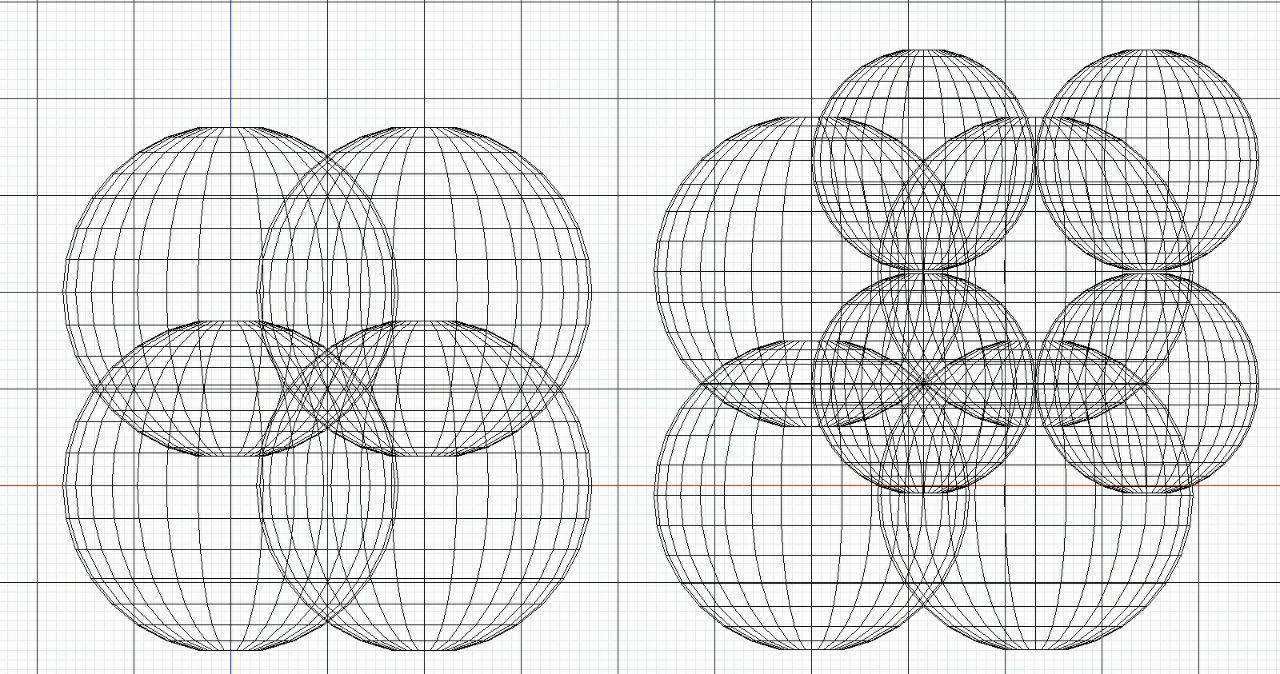
\includegraphics[width=1\textwidth]{figs/sphere_alignment_cc}
  \caption{The Alignment of the spheres\\
  Left: The perfect alignment covering the complete space\\
  Right: A previously generated alignment using small spheres to cover the missing space
  }
  \label{sphere_alignment}
\end{figure}

\subsubsection{Calculate the forces acting on the spheres}

In order to reduce the time that is needed to calculate the forces inbetween
the stars, the stars are subdivided in different cells, in this case spheres.
After all the forces acing inside one sphere are calculated, the forces are
combined and applied to the midpoint of the sphere genrating a new coordinate:
the mean force. The mean force inbetween all the cells can be calculated.

[Include description binary tree]

[Include graphic binary tree]

\subsubsection{Calculate the forces acting on all the spheres together}

This should be 0.

\subsubsection{Benchmarks}

\begin{tabular}{l | l | l | l}
  Nr of Stars & Sample rate & Galaxy Range & Time (s) \\\hline


  100         & 1           & 100          & 0.0814 \\
  75          & 1           & 100          & 0.0499 \\
  50          & 1           & 100          & 0.0295 \\
  25          & 1           & 100          & 0.0116 \\ \hline

  100         & 1           & 100          & 0.0828 \\
  100         & 2           & 100          & 0.0909 \\
  100         & 4           & 100          & 0.1832 \\
  100         & 8           & 100          & 1.1114 \\
  100         & 16          & 100          & 7.6944 \\
  100         & 32          & 100          & 56.5731 \\
  100         & 64          & 100          & 217.7768 \\ \hline

  100         & 1           & 1            & 0.0809 \\
  100         & 1           & 2            & 0.0844 \\
  100         & 1           & 4            & 0.0782 \\
  100         & 1           & 8            & 0.0758 \\
  100         & 1           & 16           & 0.0847 \\
  100         & 1           & 32           & 0.0815 \\
  100         & 1           & 64           & 0.0770 \\

\end{tabular}

The sample rate is the factor that influences the time the most. Knowing this,
it (the sample rate) can be used to controll the time in which a galaxy can
be created.
This is usefull in particular when using some very powerfull mashine with
limited time.

\subsection{Calculate the Position of a Star after a timestep}

Not to be considered:
\begin{itemize}
  \item drag
  \item any kind of resistance
  \item acceleration
\end{itemize}

\subsection{Notes}

\begin{itemize}
  \item Don't search for spheres very far away!
\end{itemize}

\begin{equation}
  % \sum_{lower}^{upper} + \sum_{lower}^{upper} - \sum_{lower}^{upper}
  \sum A_{fi} + \sum B_{fi} - \sum AB_{fij}
\end{equation}

\begin{itemize}
  \item USE dictionaries to store which stars are in wich spheres
\end{itemize}

\subsection{exec.py}

The exec.py file is used to execute the galaxytools defined in galaxytools.py.

\subsubsection{Importing the galaxytools}

\begin{lstlisting}
  import galaxytools as galaxytools
\end{lstlisting}

The complete prgramm is compressed into one object. This Object has to be
imported in order to be used.

\subsubsection{Generate a new galaxy}

\begin{lstlisting}
  galaxy = galaxytools.new_galaxy(100)
\end{lstlisting}

Using the previously imported library, one can start building a galaxy by
calling the function new\_galaxy(...). The parameter inside the braces defines
the size of the galaxy.

\subsubsection{Generate new stars in the galaxy}

\begin{lstlisting}
  galaxy.gen_new_stars(100)
\end{lstlisting}

The function new\_stars(...) is used to generate in given amount of new stars.

\subsubsection{Print the coordinates of every star in the galaxy relative to
the origin}

\begin{lstlisting}
  galaxy.print_stars()
\end{lstlisting}

Printing the coordinates of every star in the galaxy is useful for debugging:
It is clearly visible if something is going wrong on the first look. The
range of the galaxy might be wrong or the whole galaxy might be completely
wrong scaled.

\subsubsection{Calculate the forces acting inbetween all the stars in the
galaxy}

\begin{lstlisting}
  galaxy.calc_all_forces()
\end{lstlisting}

the function calc\_all\_forces() if used to calculate all the forces acting
in the selected galaxy. The O notation for this can be calculated using the
following equation: \( O(n) = n^2 \).

\subsubsection{Print the individual forces acting on the stars}

\begin{lstlisting}
  galaxy.print_individual_forces()
\end{lstlisting}

The individual forces (x, y, z) acting on the star can be printed out too!
Just use the function print\_individual\_forces() and you will recieve the
individual forces nicley formatted.

\subsubsection{Generate the coordinates of the positions for the spheres}

\begin{lstlisting}
  galaxy.gen_sphere_positions(2)
\end{lstlisting}

To generate the sphere positions subdividing the galaxy, the
gen\_sphere\_positions(...) function is utilized. The Parameter defines how
many spheres are generated on one axis of the galaxy, so a higher value equals
more spheres and so a longer time to compute. An infinite high value can be used
if the value between each star should be calculated (use at own risk!).

\subsubsection{Calculate the forces after 1 time step}

\begin{lstlisting}
  galaxy.gen_forces_after_t(1)
\end{lstlisting}

Calculating the new position after one timestep makes it possible to animate
the galaxy and so visualizing it in an exciting way making people think you've
done something awesome! This can be acchieved by using the
gen\_forces\_after\_t(...) function. It uses a timestep as an argument and
uses it to calculate the new coordinates of the star.

\subsection{galaxytools.py}

Inside this file, pretty much everything for building a galaxy is defined.

\subsubsection{Importing important libraries}

\begin{lstlisting}
# Import libraries
import math as math  # general math
import numpy as np  # advanced math
# import matplotlib.pyplot as plt  # plotting things
\end{lstlisting}

This part of the code is used to import libraries which are then used to do
e.g. advanced math.

\subsubsection{Generating the new\_galaxy class}

\begin{lstlisting}
# class used to create galaxies
class new_galaxy(object):
\end{lstlisting}

The class definition defines the galaxytools classname as new\_galaxy

\subsubsection{Initialisation}

\begin{lstlisting}

    # Initialisation
    def __init__(self, galaxy_range):
        print(
            """>>> Initialising the list storing coordinates, forces and other
            values"""
        )

        # list used for storing the coordinates os the stars
        self.list_coords = []

        # list storing the overall force acting on one star
        self.list_force_star = []

        # list storing the coordinates of the midpoints of the spheres dividing
        # the galaxy into equaly big sized cells
        self.list_sphere_coords = []

        # self.list_sphere_stars = np.array(3, )

        print("\tDone\n")
        print(">>> Initialising variables and constants")

        # variable storing the number of stars generated
        self.num_of_stars = 0

        self.galaxy_range = int(galaxy_range)

        # define the universal gravitational constant
        self.G = 6.67408 * 10e11

        print("\tDone\n")

\end{lstlisting}

\subsubsection{Generating new stars}

\begin{lstlisting}

    # generate n new stars and store the coordinates in list_coords
    # n = number of stars to be generated
    # galaxy_range = size of the galaxy
    def gen_new_stars(self, n):
        print(">>> Generating Stars...")

        # for a given number of stars
        for i in range(0, n):

            # generate a temporary random coordinate inside a given range using
            # numpy
            self.temp_coord = np.random.uniform(
                low=0, high=self.galaxy_range, size=(4, ))

            # append the random coordinate to the list storing the coordinates
            self.list_coords.append(self.temp_coord)

        # increment the generated star counter
        self.num_of_stars += n
        print("\tDone")
        print("\tGenerated " + str(n) + " Stars\n")

\end{lstlisting}

\subsubsection{Print out all the star coordinates}

\begin{lstlisting}

    # print out all the coordinates in list_coords
    def print_stars(self):
        print(">>> Listing the coordinates of all stars:")
        # print the coordinates of every star
        for value in self.list_coords:
            print(value)

        print("\tDone\n")

\end{lstlisting}

\subsubsection{Calculate the forces acting inbetween two stars}

\begin{lstlisting}

    # calculate the forces acting between two stars on a specified axis
    # star1 = coordinates of the first star
    # star2 = coordinates of the second star
    # axes = "x", "y" or "z" (CASE SENSITIVE!)
    def calc_forces(self, star1, star2, axes):
        if axes == "x":
            mass = star1[3] * star2[3]
            distance = math.sqrt(math.pow(star1[0] - star2[0], 2))
        elif axes == "y":
            mass = star1[3] * star2[3]
            distance = math.sqrt(math.pow(star1[1] - star2[1], 2))
        elif axes == "z":
            mass = star1[3] * star2[3]
            distance = math.sqrt(math.pow(star1[2] - star2[2], 2))

        # stop division by zero
        if distance == 0:
            pass
        else:
            # return the acting force
            return self.G * mass / math.pow(distance, 2)

\end{lstlisting}

\subsubsection{Calculate all the forces acting in the galaxy}

\begin{lstlisting}

    # calculate all the forces acting in the current galaxy
    def calc_all_forces(self):
        print(">>> Calculating all the forces acting inbetween the stars:")

        if (self.num_of_stars <= 5):
            # print some information above the columns
            print(">>> Printing the forces acting inbetween every star")
            print("{:-<60}".format(""))
            print("\t| {:<3}| {:<3}| ".format("a", "b"))
            print("\t+{:-<4}+{:-<4}+{:-<60} ".format("", "", ""))

        else:
            print("\t[W] Too many stars to print out!")
            print("{:-<60}".format(""))

        # for every star
        for i in range(0, self.num_of_stars):

            # initialize
            self.force = 0

            # every other star:
            for j in range(0, self.num_of_stars):

                # don't calculate the force between a star and and itself
                if i != j and i < j:
                    self.arr_force = np.array((0, 0, 0))

                    # calculate the force between the two stars
                    force_x = self.calc_forces(self.list_coords[i],
                                               self.list_coords[j], "x")
                    force_y = self.calc_forces(self.list_coords[i],
                                               self.list_coords[j], "y")
                    force_z = self.calc_forces(self.list_coords[i],
                                               self.list_coords[j], "z")

                    # print("overall force: ", end="")
                    self.arr_force = np.array((force_x, force_y, force_z))

                    if (self.num_of_stars <= 5):
                        print("\t| {:<3}| {:<3}| {:<60}".format(
                            str(i), str(j), str(self.arr_force)))
                    """
                    force_x = 42
                    force_y = 36
                    force_z = 24

                    (0, 0, 0) --> (42, 36, 24)
                    """

            # append the variable to the list storing all the forces
            self.list_force_star.append(self.arr_force)

        print("{:-<60}".format(""))
        print("\tDone\n")

\end{lstlisting}

\subsubsection{Print the individual forces acting on one star}

\begin{lstlisting}

    # print the individual forces acting on a star
    def print_individual_forces(self, n=None, print_confirm=False):
        print(">>> Printing the individual forces acting on every star")

        if self.num_of_stars > 10:
            print("\t[W] Too many stars to print out!")
            print("{:-<60}".format(""))

            for i in range(0, 3):
                print("\t" + str(i) + " " + str(self.list_force_star[i]))

            print("\n\t...\n")

            for i in range(
                    int(len(self.list_force_star) - 3),
                    len(self.list_force_star)):
                print("\t" + str(i) + " " + str(self.list_force_star[i]))
            print("{:-<60}".format(""))

        else:
            print("{:-<60}".format(""))
            if n is None:
                # for value in self.list_force_star:
                for i in range(0, len(self.list_force_star)):
                    print("\t" + str(i) + " " + str(self.list_force_star[i]))
            else:
                print(self.list_force_star[n])

            print("{:-<60}".format(""))
            print("\tDone\n")

\end{lstlisting}

\subsubsection{Find out if a star is inside one sphere}

\begin{lstlisting}

    # star      [x, y, z, mass]
    # sphere    [x, y, z, radius]
    def is_star_in_sphere(self, star, sphere):

        # define the sphere values
        self.sphere_x = sphere[0]
        self.sphere_y = sphere[1]
        self.sphere_z = sphere[2]
        self.sphere_r = sphere[3]

        # define the star coordinates
        self.star_x = star[0]
        self.star_y = star[1]
        self.star_z = star[2]

        # find out the distance between the point and the center of the sphere
        # if the distance is bigger than the radius of the sphere, the point is
        # not inside the sphere. Elsewise, the point is inside the sphere

        x = math.pow(self.sphere_x - self.star_x, 2)
        y = math.pow(self.sphere_y - self.star_y, 2)
        z = math.pow(self.sphere_z - self.star_z, 2)
        r = math.sqrt(x + y + z)

        if r > self.sphere_r:
            return False
        else:
            return True

        # self.sphere_x_neg = self.sphere_x - self.sphere_r
        # self.sphere_x_pos = self.sphere_x + self.sphere_r
        #
        # self.sphere_y_neg = self.sphere_y - self.sphere_r
        # self.sphere_y_pos = self.sphere_y + self.sphere_r
        #
        # self.sphere_z_neg = self.sphere_z - self.sphere_r
        # self.sphere_z_pos = self.sphere_z + self.sphere_r
        #
        # # find out if the star is inside the sphere
        # if self.sphere_x_neg < self.star_x < self.sphere_x_pos:
        #     if self.sphere_y_neg < self.star_y < self.sphere_y_pos:
        #         if self.sphere_z_neg < self.star_z < self.sphere_z_pos:
        #             return True
        #         else:
        #             return False
        #     else:
        #         return False
        # else:
        #     return False

\end{lstlisting}

\subsubsection{Find out which star in in which spheres}

\begin{lstlisting}

    # find out which stars in in which spheres
    def is_star_in_sphere_all(self):

        # print(self.sphrer_rs)

        print(">>> is_star_in_sphere_all")

        # initialize a temporary counter in order to index the spheres
        tmp_counter = 0

        # cycle through all the stars
        for sphere in self.sphere_coords:
            # print("sphere: " + str(sphere))

            tmp_list = []
            for star in self.list_coords:
                # parse the needed values from the sphere list

                # if the star is inside the sphere
                if (self.is_star_in_sphere(star, sphere) is True):
                    # print("\nstar: " + str(star))

                    star_x = []

                    for value in star:
                        # print(value, end=" ")
                        # print("")
                        star_x.append(value)

                    # print("star_x :" + str(star_x))

                    tmp_list.append(star_x)

            # print("")
            # print("tmp_list: " + str(tmp_list))
            # print("END")

            self.sphere_coords[sphere] = tmp_list

        print("")
        # print(self.sphere_coords)

        # cycle through the dictionary storing which star is in which cell
        for value in self.sphere_coords:
            stars_in_sphere = self.sphere_coords[value]

            # calculate the individual forces in the sphere
            self.calc_forces_sphere(stars_in_sphere)

            # for value in stars_in_sphere:
                # print(value)

\end{lstlisting}

\subsubsection{Generate the sphere positions}

\begin{lstlisting}

    # function generating the positions of the sphere cells
    def gen_sphere_positions(self, sampling_rate):

        print(">>> Generating the sphere positions")

        # initialize a dictionary linking the sphere coordinates to the
        # coordiantes of the stars in the sphere
        self.sphere_coords = {}

        # calculate the distance between the midpoints of the spheres
        sphere_distance = int(round(self.galaxy_range / sampling_rate, 0))

        # define the sphere_radius
        tmp_var = math.pow(sphere_distance, 2)
        sphere_radius = math.sqrt(tmp_var + tmp_var + tmp_var)

        # define a sphere counter for "labeling" the spheres
        tmp_counter = 0

        # cycle through all potential points
        for i in range(-self.galaxy_range, self.galaxy_range, sphere_distance):
            for j in range(-self.galaxy_range, self.galaxy_range,
                           sphere_distance):
                for k in range(-self.galaxy_range, self.galaxy_range,
                               sphere_distance):

                    # generate a temporary array combining all values
                    # temp_arr = np.array((i, j, k, sphere_radius, tmp_counter))
                    tmp_arr = (i, j, k, sphere_radius, tmp_counter)

                    # append the array to the list storing the sphere infos
                    # self.list_sphere_coords.append(temp_arr)

                    # print("temp_arr: " + str(temp_arr))
                    self.sphere_coords[tmp_arr[0:4]] = []

                    # increment the sphere counter
                    tmp_counter += 1

        # print(self.sphere_coords)
        print("\tDone\n")

\end{lstlisting}

\subsubsection{Calculate the forces acting inside the sphere}

\begin{lstlisting}

    def calc_forces_sphere(self, stars_in_sphere):
        print("stars_in_sphere: ", end="")
        print(stars_in_sphere)
        # for value in stars_in_sphere:
        #     self.calc_all_forces(stars_in_sphere)
        #     print(value)

\end{lstlisting}

\subsubsection{calculate the forces acting in every sphere}

\begin{lstlisting}

    def calc_forces_sphere_all():
        # for i in range(0, len(num_of_spheres)):
        #     for star in sphere[i]:
        #         for star_2 in len(0, num_of_stars_in_sphere[i])
        #             a = calc_force(star, star[j])

        pass

    def gen_print_forces_after_t(t):
        pass

    # def all_stars_in_sphere(self, star, se)

\end{lstlisting}

\subsection{GAN}

\include*{docs/6_abgabe}

\end{document}
